\documentclass{standalone}
\usepackage{tikz}
\usetikzlibrary{decorations.pathreplacing,decorations.pathmorphing}
\usetikzlibrary{fit,quotes}
\usepackage{yquant, braket}

\begin{document}

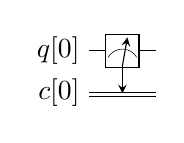
\begin{tikzpicture}[scale=1.000000,x=1pt,y=1pt]
\filldraw[color=white] (0.000000, -7.500000) rectangle (24.000000, 22.500000);
% Drawing wires
% Line 2: q0 W q[0]
\draw[color=black] (0.000000,15.000000) -- (12.000000,15.000000);
\draw[color=black] (12.000000,15.00000) -- (24.000000,15.00000);
% \draw[color=black] (12.000000,15.500000) -- (24.000000,15.500000);
\draw[color=black] (0.000000,15.000000) node[left] {$q[0]$};
% Line 3: c0 W c[0]
\draw[color=black] (0.000000,0.000000) -- (24.000000,0.000000);
\draw[color=black] (0.000000,-1.5000000) -- (24.000000,-1.5000000);
\draw[color=black] (0.000000,0.000000) node[left] {$c[0]$};
% Done with wires; drawing gates
% Line 4: q0:cwire +c0 %% or
%\draw (30.000000, 13.00000) node[text width=144pt,below,text centered] {\scriptsize or};
% \draw (11.500000,15.000000) -- (11.500000,0.000000);
 \draw (12.00000,15.000000) -- (12.00000,0.000000);
%\filldraw (12.000000, 15.000000) circle(1.500000pt);
\begin{scope}
%\draw[fill=white] (12.000000, 0.000000) circle(3.000000pt);
 \clip (12.000000, 0.000000) circle(3.000000pt);
\draw (9.000000, 0.000000) -- (15.000000, 0.000000);
% \draw (12.000000, -3.000000) -- (12.000000, 3.000000);
\end{scope}
\draw[fill=white] (6.000000, 9.000000) rectangle (18.000000, 21.000000);
\draw[very thin] (12.000000, 15.600000) arc (90:150:6.000000pt);
\draw[very thin] (12.000000, 15.600000) arc (90:30:6.000000pt);
\draw[->,>=stealth] (12.000000, 9.600000) -- +(80:10.392305pt);
\draw[->,>=stealth] (12.000000, 10.00000)  -- +(270:10.392305pt); % arrowhead
% Done with gates; drawing ending labels
% Done with ending labels; drawing cut lines and comments
% Done with comments
\end{tikzpicture}
\end{document}
